\documentclass[compress]{beamer}
\usepackage{ifthen,verbatim,hyperref}

\newcommand{\isnote}{}
\xdefinecolor{lightyellow}{rgb}{1.,1.,0.25}
\xdefinecolor{darkblue}{rgb}{0.1,0.1,0.7}

%% Uncomment this to get annotations
%% \def\notes{\addtocounter{page}{-1}
%%            \renewcommand{\isnote}{*}
%% 	   \beamertemplateshadingbackground{lightyellow}{white}
%%            \begin{frame}
%%            \frametitle{Notes for the previous page (page \insertpagenumber)}
%%            \itemize}
%% \def\endnotes{\enditemize
%% 	      \end{frame}
%%               \beamertemplateshadingbackground{white}{white}
%%               \renewcommand{\isnote}{}}

%% Uncomment this to not get annotations
\def\notes{\comment}
\def\endnotes{\endcomment}

\setbeamertemplate{navigation symbols}{}
\setbeamertemplate{headline}{\mbox{ } \hfill
\begin{minipage}{5.5 cm}
\vspace{-0.75 cm} \small
\end{minipage} \hfill
\begin{minipage}{4.5 cm}
\vspace{-0.75 cm} \small
\begin{flushright}
\ifthenelse{\equal{\insertpagenumber}{1}}{}{Jim Pivarski \hspace{0.2 cm} \insertpagenumber\isnote/\pageref{numpages}}
\end{flushright}
\end{minipage}\mbox{\hspace{0.2 cm}}\includegraphics[height=1 cm]{../cmslogo} \hspace{0.1 cm} \includegraphics[height=1 cm]{../tamulogo} \hspace{0.01 cm} \vspace{-1.05 cm}}

\begin{document}
\begin{frame}
\vfill
\begin{center}
\textcolor{darkblue}{\Large Magnetic Field from a Muon Alignment Perspective}

\vfill
\begin{columns}
\column{0.3\linewidth}
\begin{center}
\large
\textcolor{darkblue}{Jim Pivarski}

\vspace{0.2 cm}
Alexei Safonov
\end{center}
\end{columns}

\begin{columns}
\column{0.3\linewidth}
\begin{center}
\scriptsize
{\it Texas A\&M University}
\end{center}
\end{columns}

\vfill
 2 February, 2009

\end{center}
\end{frame}

%% \begin{notes}
%% \item This is the annotated version of my talk.
%% \item If you want the version that I am presenting, download the one
%% labeled ``slides'' on Indico (or just ignore these yellow pages).
%% \item The annotated version is provided for extra detail and a written
%% record of comments that I intend to make orally.
%% \item Yellow notes refer to the content on the {\it previous} page.
%% \item All other slides are identical for the two versions.
%% \end{notes}

\small

\begin{frame}
\frametitle{Entangled problems?}
\begin{itemize}\setlength{\itemsep}{0.25 cm}
\item The alignment of the muon chambers and the distribution of
  magnetic field are both imperfectly known
\item Both cause deviations in muon trajectories with respect to
  tracks propagated from the tracker
\item How can they be distinguished?
\begin{itemize}\setlength{\itemsep}{0.1 cm}
\item residuals from misalignment are independent of track momentum and charge
\item residuals from $\vec{B}$-field mismodelling depends on momentum and is antisymmetric with charge
\end{itemize}
\item This talk will be about exploiting the above to
\begin{itemize}\setlength{\itemsep}{0.1 cm}
\item align the DT chambers
\item verify $\vec{B}$-field error calculations using techniques developed for alignment
\end{itemize}
\end{itemize}
%% \hspace{-0.83 cm} \textcolor{darkblue}{\Large Outline2}
\end{frame}

\begin{frame}
\frametitle{Basic alignment technique}
\begin{columns}
\column{0.35\linewidth}
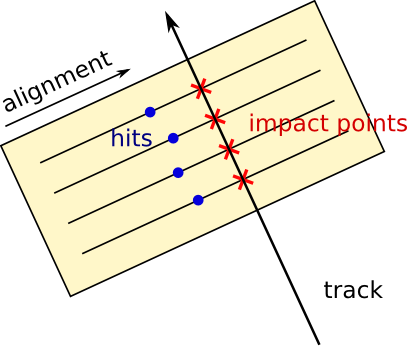
\includegraphics[width=\linewidth]{hip_explanation.png}

\column{0.65\linewidth}

\textcolor{darkblue}{HIP algorithm: ``Hits and Impact Points''}
\begin{itemize}
\item Using a track as reference, alignment correction is the peak of the residuals distribution

\item Our $\mbox{residual} \equiv \left(\mbox{impact point}\right) - \left(\mbox{hit}\right)$

\end{itemize}
\end{columns}

\vfill
Implementation is not exactly the same as that in the tracker

\begin{itemize}
\item Muon hits excluded from refitted tracks: tracker is \mbox{external reference\hspace{-1 cm}}
\begin{itemize}
\item breaks the circularity between fitting tracks and \mbox{aligning chambers\hspace{-1 cm}}
\item no need to iterate: convergence in one step
\end{itemize}
%% \item Only hits within a chamber on one track are averaged with weights
%% \begin{itemize}
%% \item handles statistics of correlated hits properly
%% \end{itemize}
\item Muon chambers are much bigger than silicon wafers: study
  residuals as a function of position throughout each chamber
\end{itemize}
\end{frame}

\begin{frame}
\frametitle{Effect of $\vec{B}$-field on residuals}

\begin{columns}
\column{0.75\linewidth}
\begin{itemize}
\item Track propagation is sensitive to the integral of $\vec{B}$-field error along its path
\item Effect on residuals flips sign with charge
\item The number of positively-charged tracks is not equal to the number of negatively-charged tracks
\item But both charges have the same \mbox{momentum distribution\hspace{-1 cm}} (a fact used in the cosmics charge ratio analysis)
\end{itemize}

\column{0.25\linewidth}
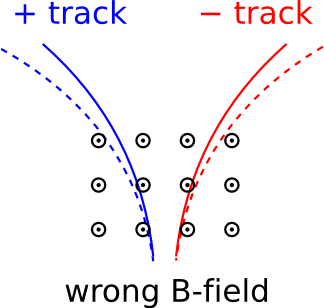
\includegraphics[width=\linewidth]{antisymmetric_bfield.png}
\end{columns}

\begin{center}
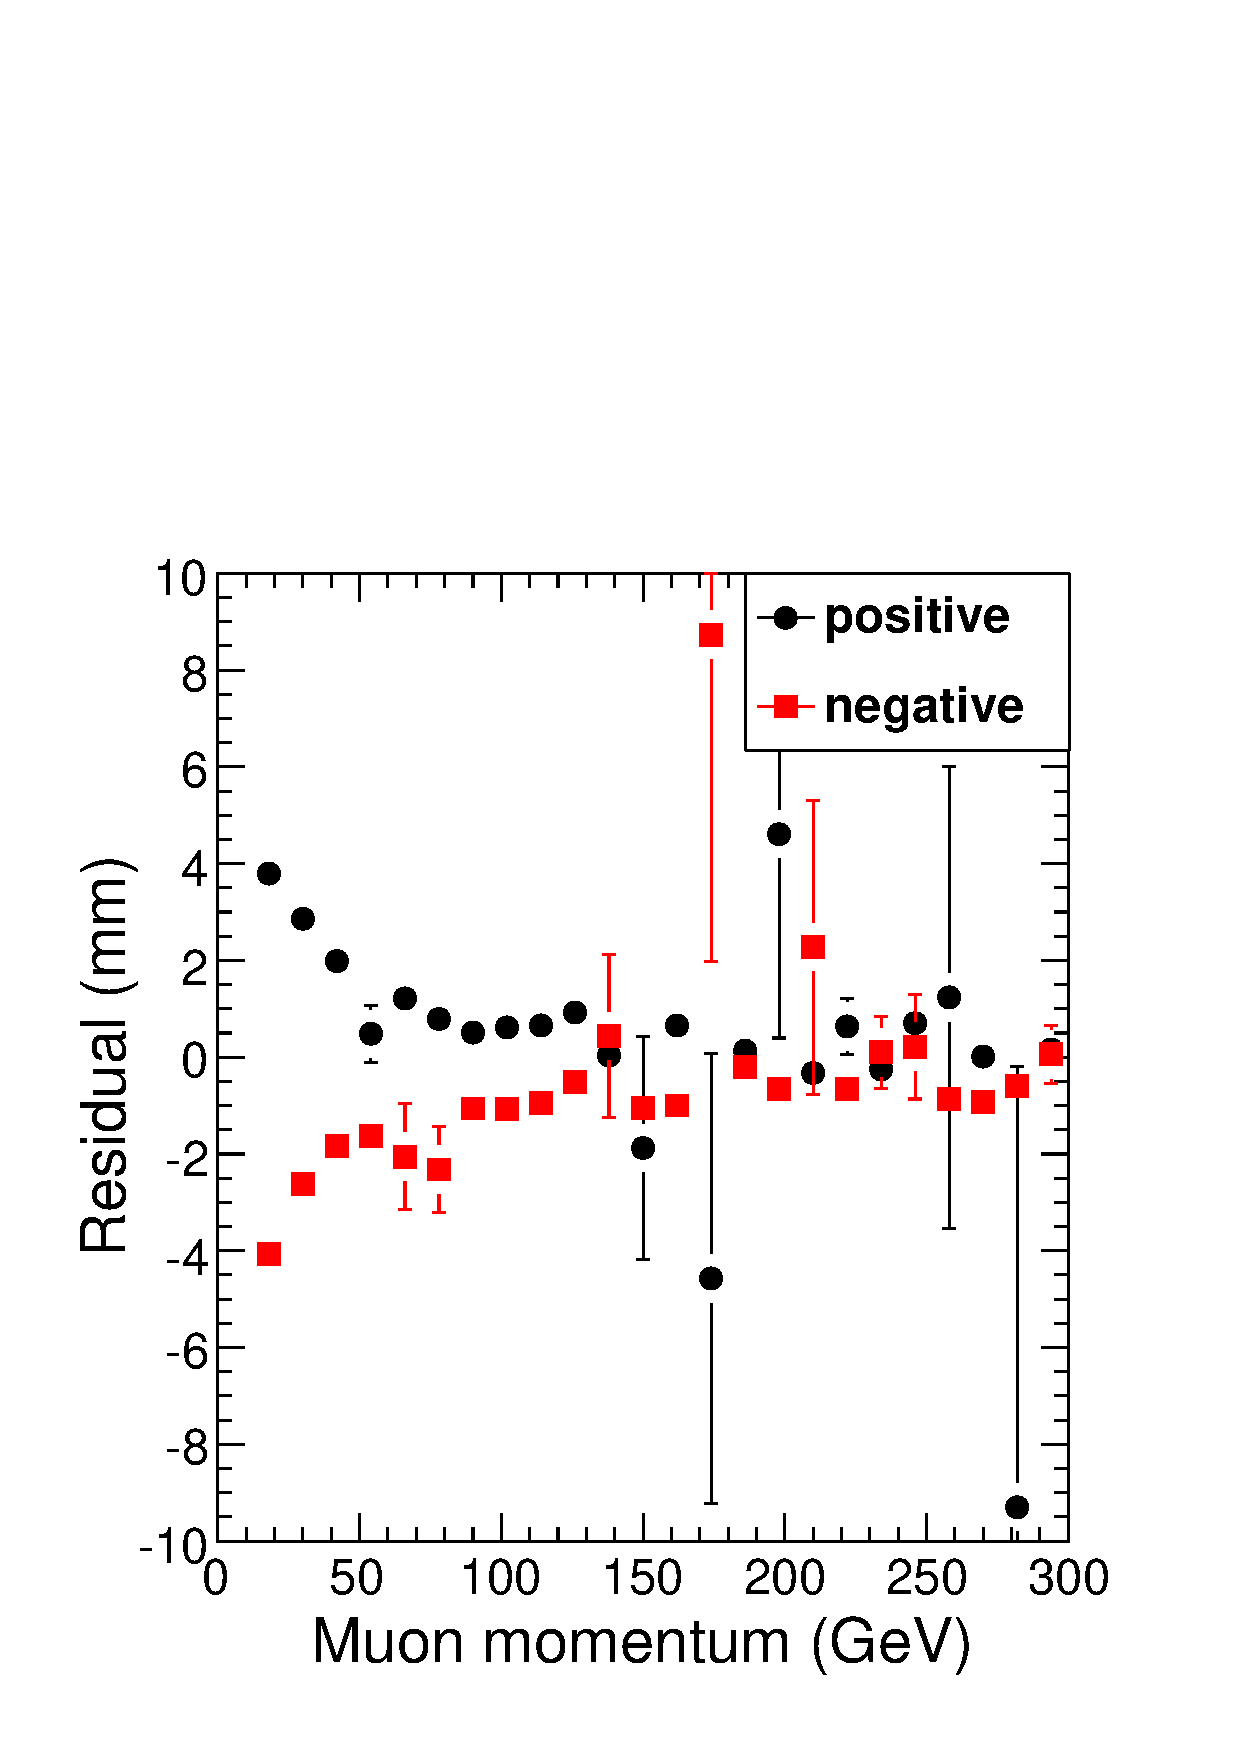
\includegraphics[height=4 cm]{demo_residual.pdf} \hspace{1 cm} 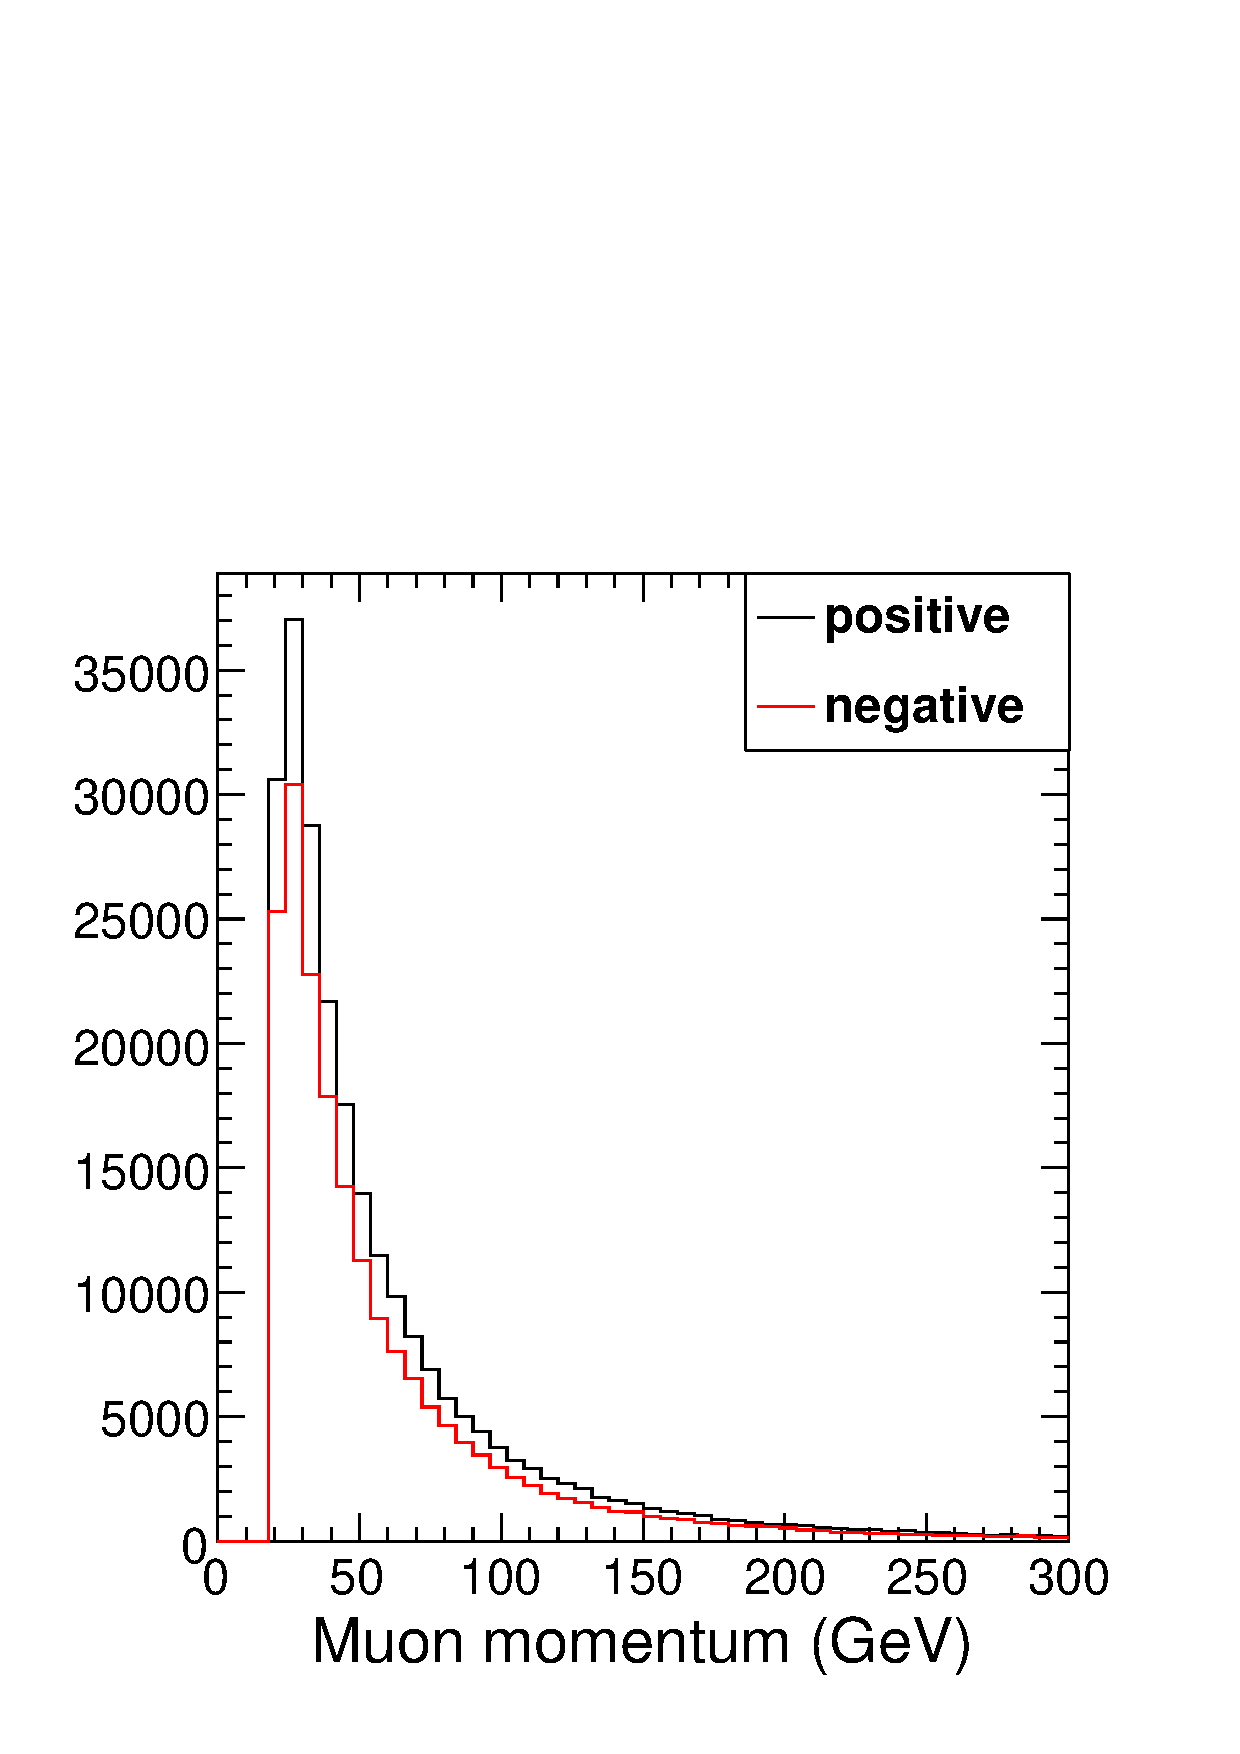
\includegraphics[height=4 cm]{demo_momentum.pdf}
\end{center}
\end{frame}

\begin{frame}
\frametitle{Controlling $\vec{B}$-error in alignment}

\vspace{0.5 cm}
\begin{columns}
\column{0.6\linewidth}
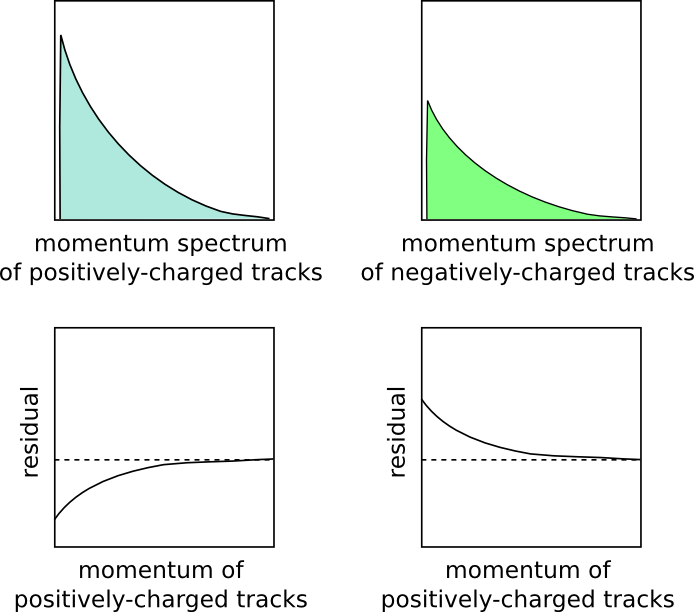
\includegraphics[width=\linewidth]{momentum_explanation.png}

\column{0.4\linewidth}
\begin{itemize}
\item Measure residuals peak in two bins, one for each charge
\item Non-weighted average is insensitive to $\vec{B}$-field errors

$\displaystyle \mbox{alignment} = \frac{R_+ + R_-}{2}$

\item Difference is maximally sensitive

$\displaystyle \mbox{error tracer} = \frac{R_+ - R_-}{2}$

\end{itemize}
\end{columns}

\begin{itemize}\setlength{\itemsep}{-0.1 cm}
\item Alignment calculation effectively scales up negatively-charged muon contribution so that the $\vec{B}$-field errors cancel
\item \mbox{$\displaystyle \mbox{Systematic error} = \left(\mbox{error tracer}\right) \times \left(\mbox{charge mismeasurement}\right) \times \frac{0.3}{2.3}$} \\
\textcolor{white}{$\mbox{Systematic error}$} $\sim \left(\mbox{error tracer}\right) \times \left(\mbox{a few percent or less}\right)$

\end{itemize}
\end{frame}

\begin{frame}
\frametitle{Demonstration in station~4}
\begin{itemize}
\item Station 4 has the largest $\vec{B}$-field mismodelling
\item The misalignment measure breaks cleanly at the \mbox{chamber boundaries\hspace{-1 cm}}
\item The tracer of $\vec{B}$-field errors is constant
\end{itemize}

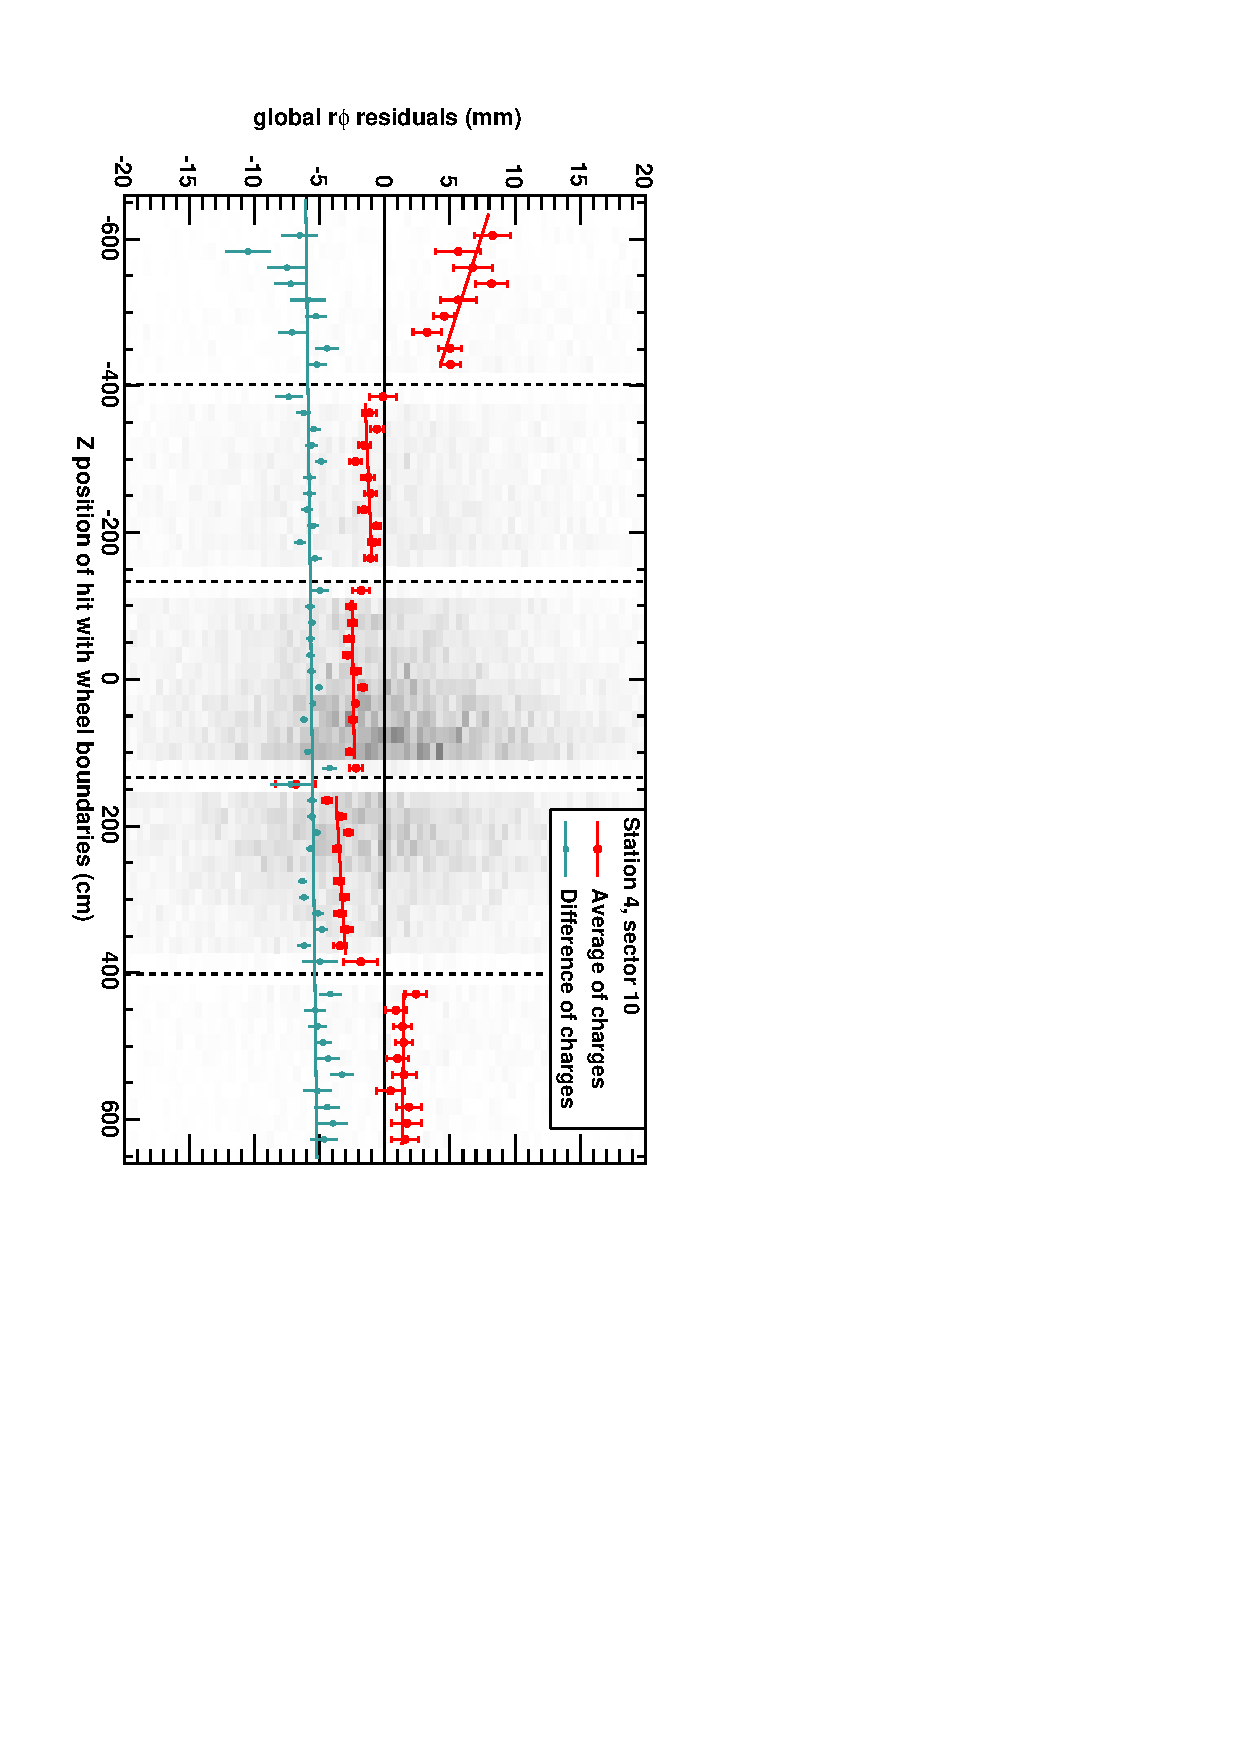
\includegraphics[height=\linewidth, angle=90]{demo_of_bfield.pdf}

\scriptsize grey background is the raw 2-D residuals distribution

linear fits are only a guide for the eye: not used in alignment!
\end{frame}

\begin{frame}
\frametitle{Alignment results}

\begin{columns}
\column{0.4\linewidth}
\begin{itemize}
\item Sample before-and-after residuals plots from alignment shown \mbox{at right\hspace{-1 cm}}
\item Complete set of 152 pages at last DT-DPG (``more information'')

\textcolor{blue}{\tt \tiny \href{http://indico.cern.ch/conferenceDisplay.py?confId=51267}{http://indico.cern.ch/}}

\vspace{-0.3 cm}
\textcolor{blue}{\tt \tiny \href{http://indico.cern.ch/conferenceDisplay.py?confId=51267}{conferenceDisplay.py?confId=51267}}

\item Aligned local $x$, $y$, $\phi_z$ for DT chambers with sufficient statistics

\item Trend in $r\phi$ residual vs.\ $\phi$ suggests DT chamber description error \\ (under investigation)

\item 5--10~mm misalignments reduced to $\mathcal{O}(\mbox{1--2~mm})$

\end{itemize}

\column{0.6\linewidth}

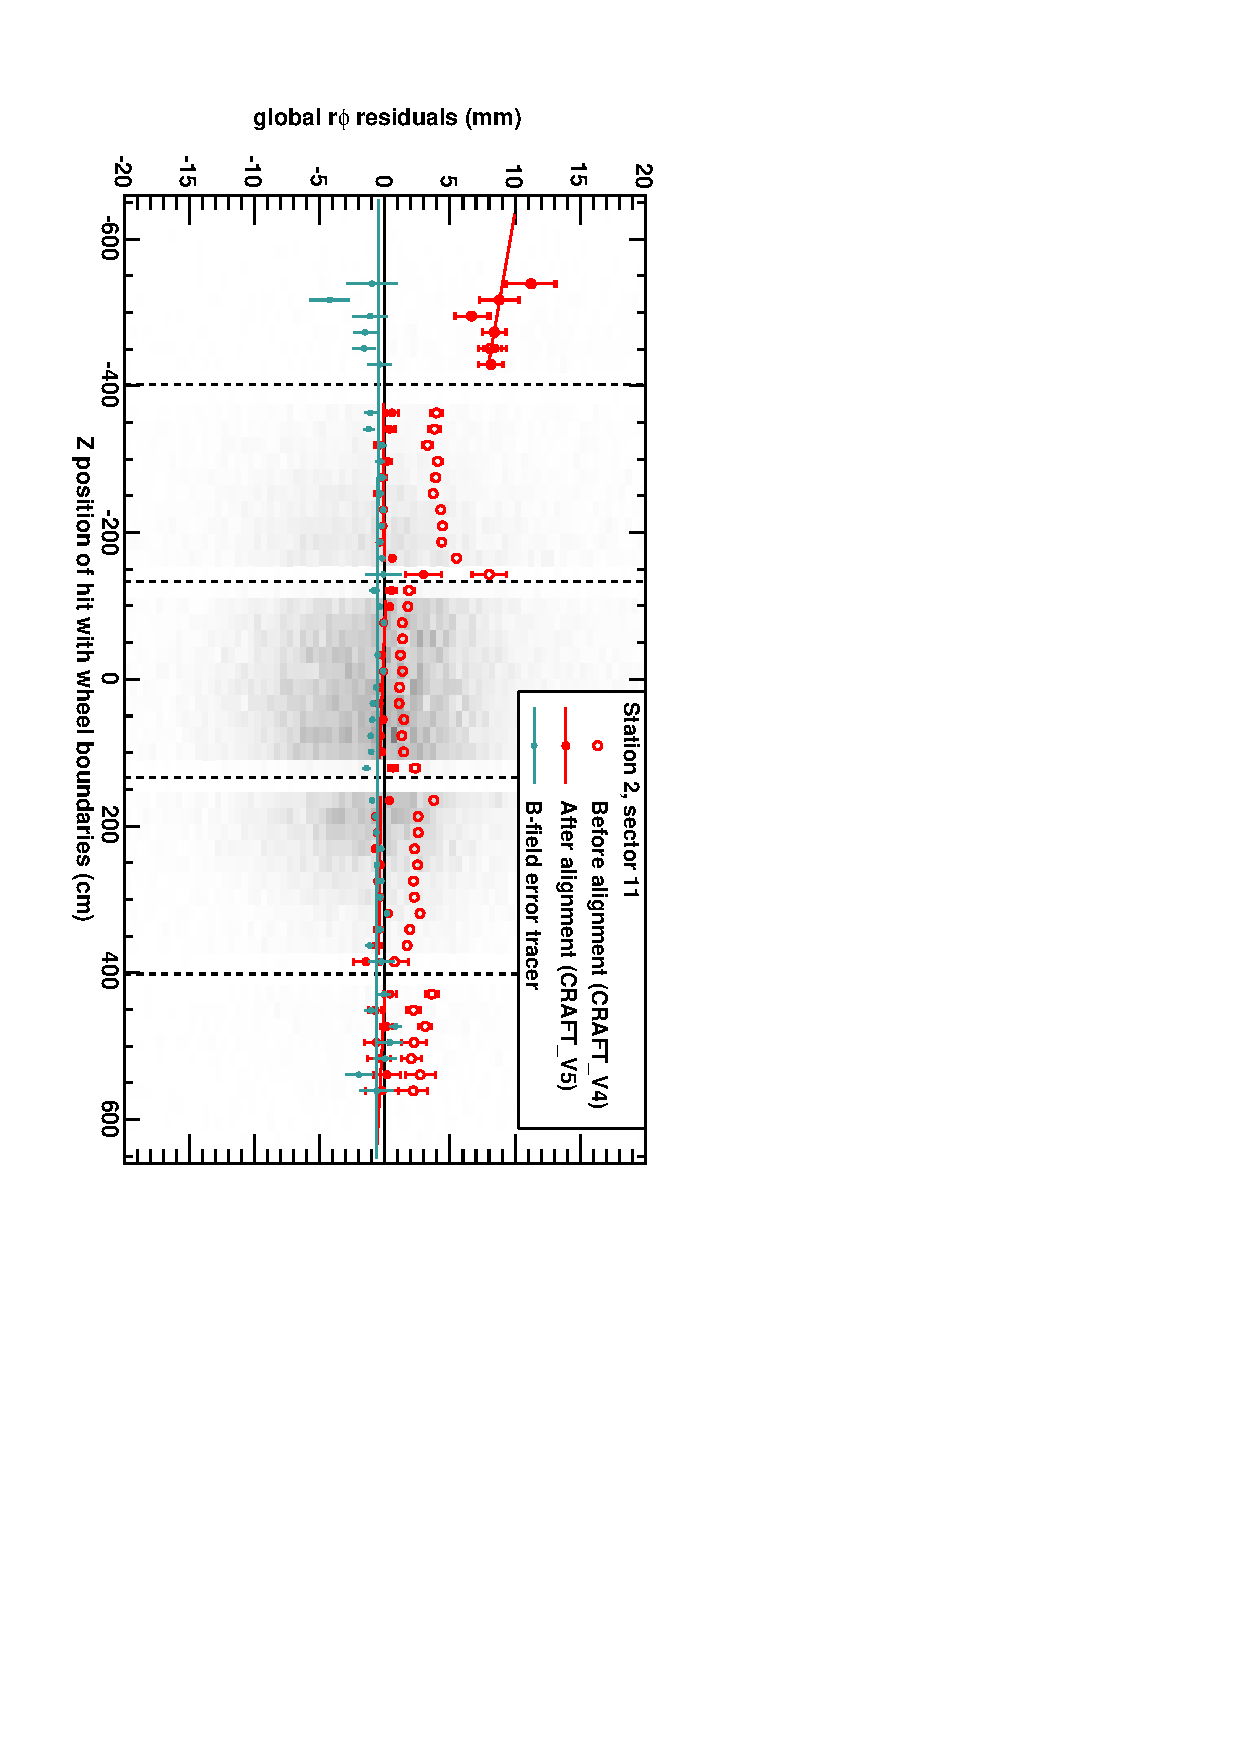
\includegraphics[height=1.1\linewidth, angle=90]{bfieldtalk_example1.pdf}

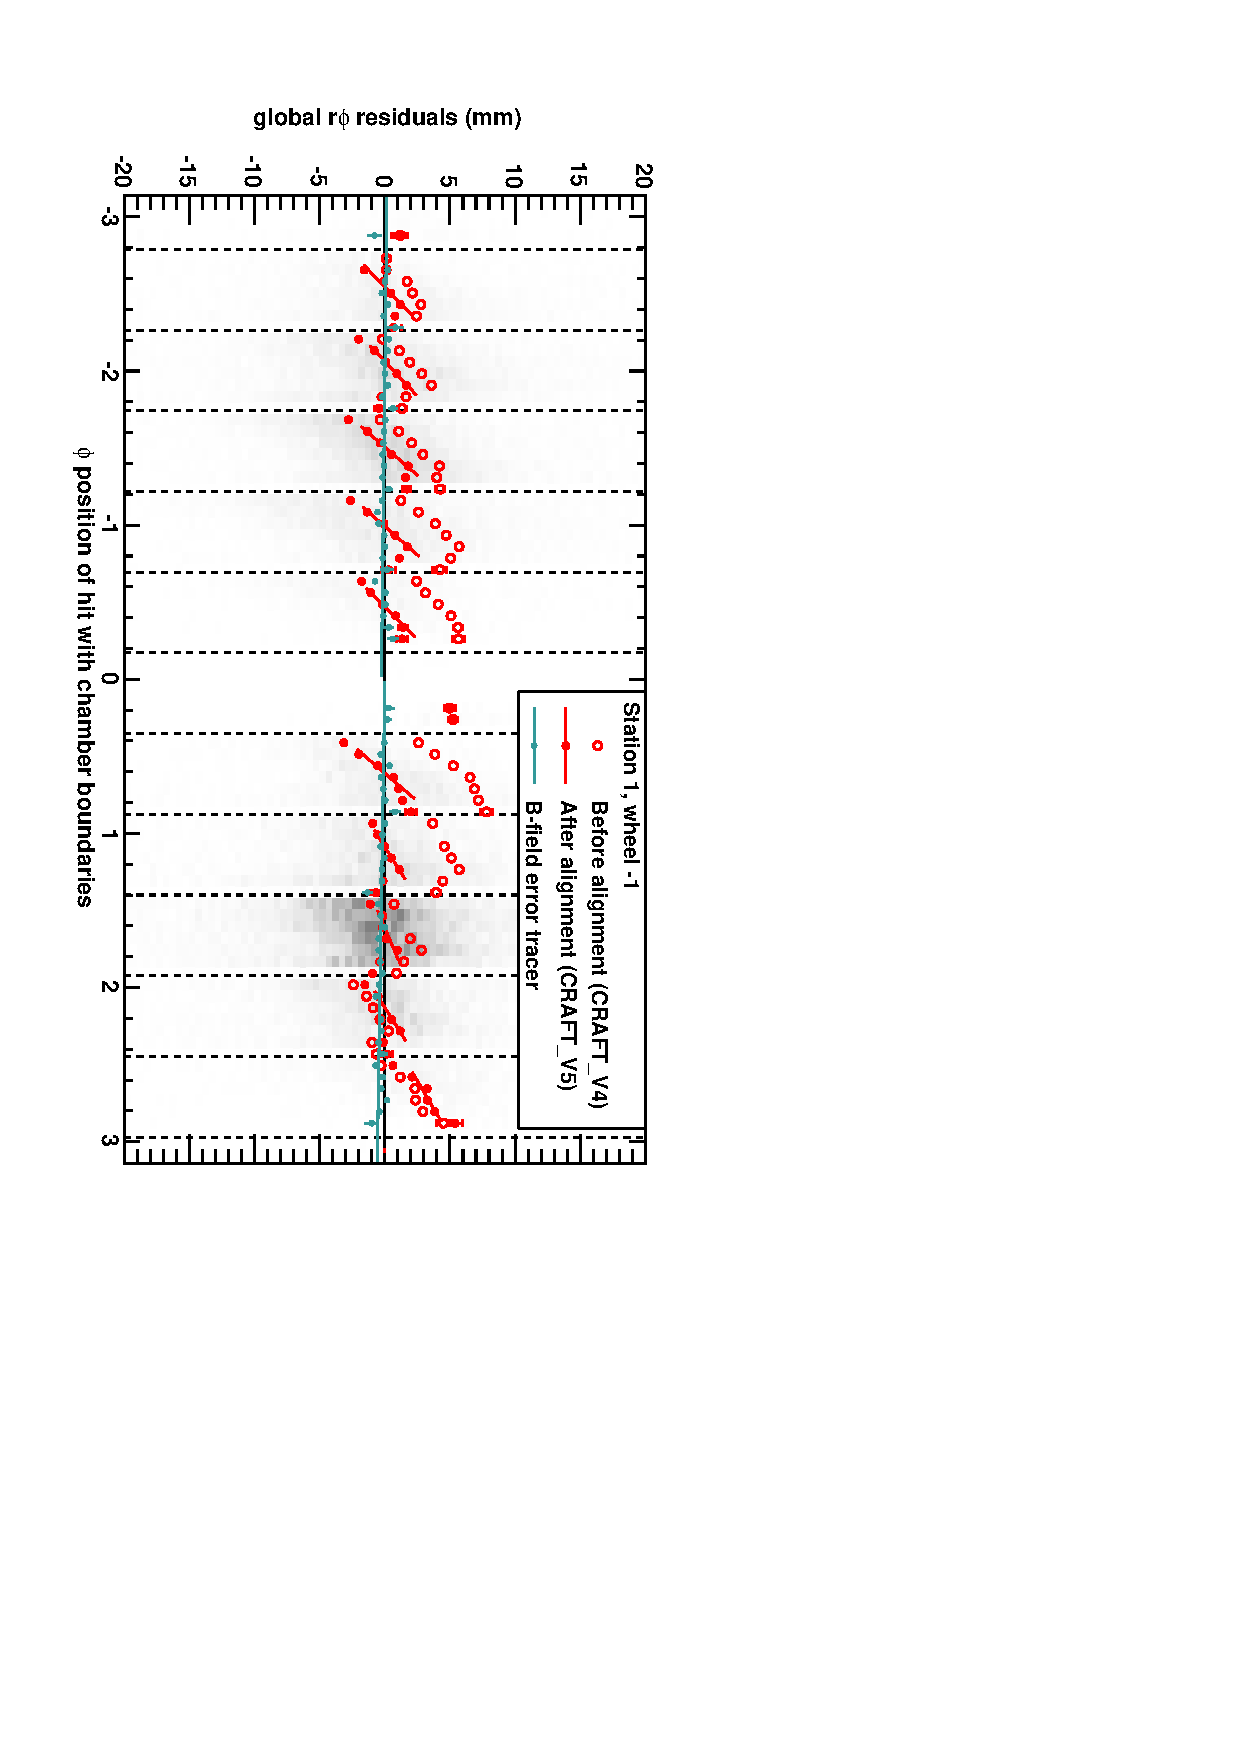
\includegraphics[height=1.1\linewidth, angle=90]{bfieldtalk_example2.pdf}

\end{columns}
\end{frame}

\begin{frame}
\frametitle{Residuals differences plots}

\vspace{0.3 cm}
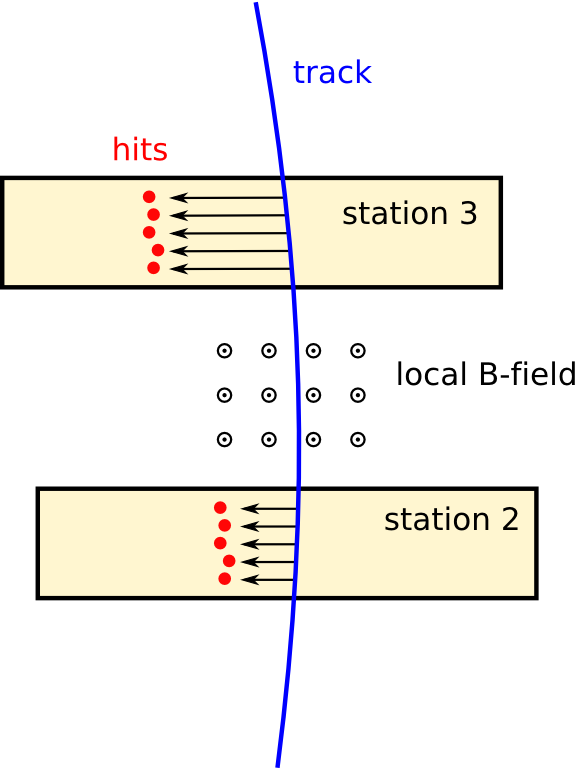
\includegraphics[height=4.4 cm]{residuals_difference.png} 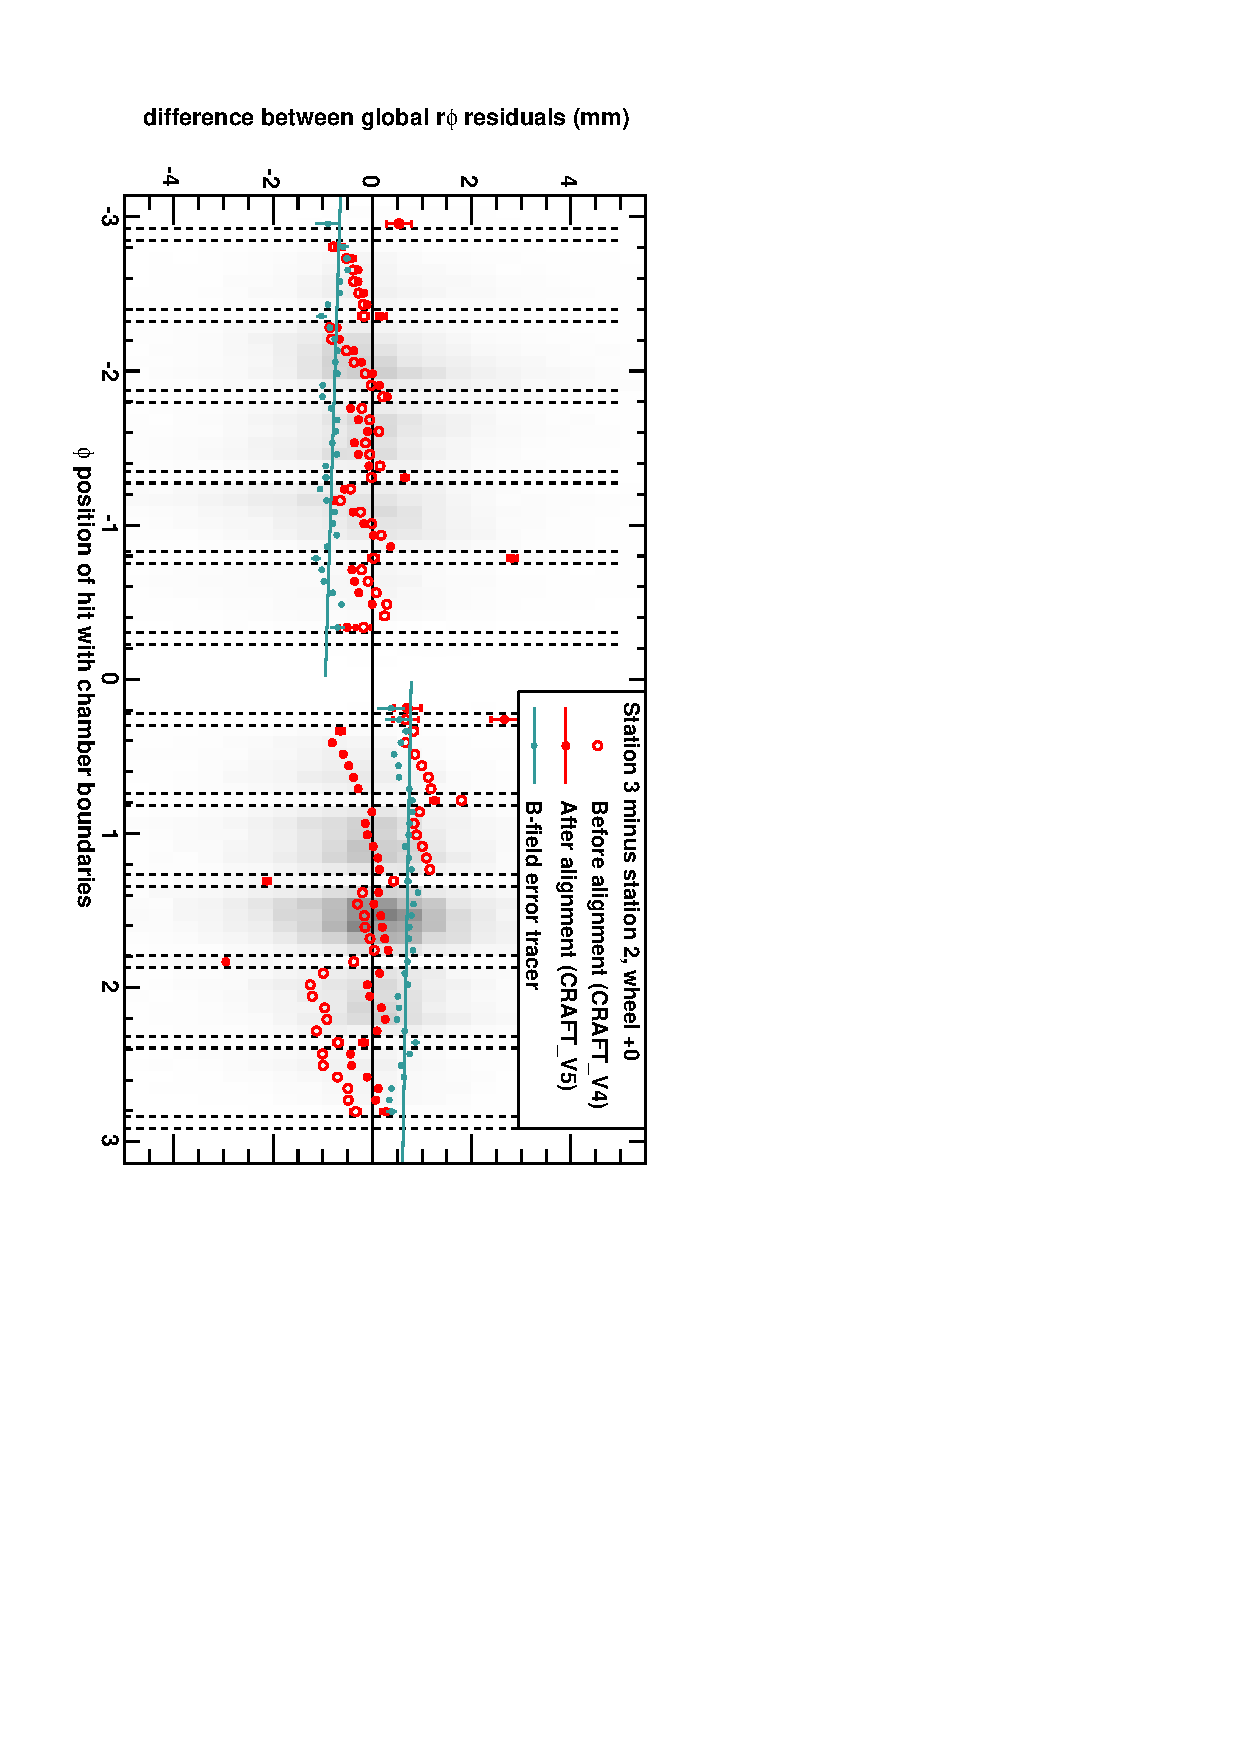
\includegraphics[width=4.5 cm, angle=90]{bfieldtalk_example4.pdf}

\vspace{-0.3 cm}
\begin{itemize}
\item Consider difference of residuals between stations on the same track:

\mbox{ } \hfill \mbox{$\mbox{difference} = \big(\mbox{st.\ 3 track} - \mbox{st.\ 3 hit}\big) - \big(\mbox{st.\ 2 track} - \mbox{st.\ 2 hit}\big)$} \hfill \mbox{ }

\item Linearly-independent cross-check on alignment because it displays relative alignment of chambers, rather than absolute position

\item Also sensitive to local $\vec{B}$-field error, rather than integral over path
\begin{itemize}
\item wrong sign in $\phi > 0$ part because cosmic muon's \mbox{velocity is down\hspace{-1 cm}}
\end{itemize}
\end{itemize}
\end{frame}

\begin{frame}
\frametitle{Calculating $B_z$ error in Tesla}

\vspace{0.3 cm}
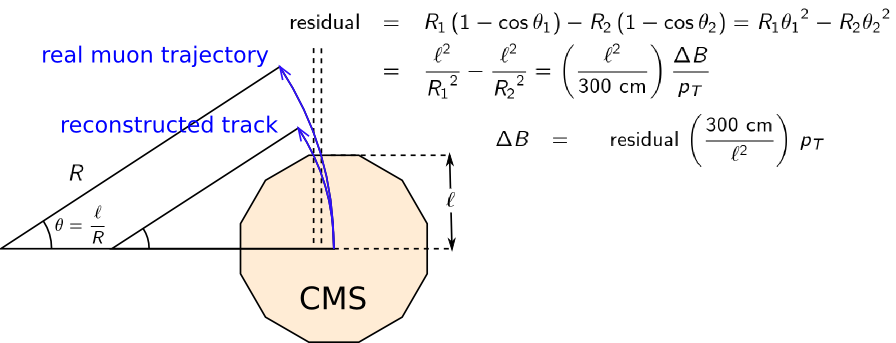
\includegraphics[width=\linewidth]{geometry.png}

\begin{columns}
\column{0.5\linewidth}
\mbox{ }

\scriptsize P.\ Martinez: $r\phi$ residual vs.\ $q/p_T$ \mbox{by station\hspace{-1 cm}}

\vspace{0.05 cm}
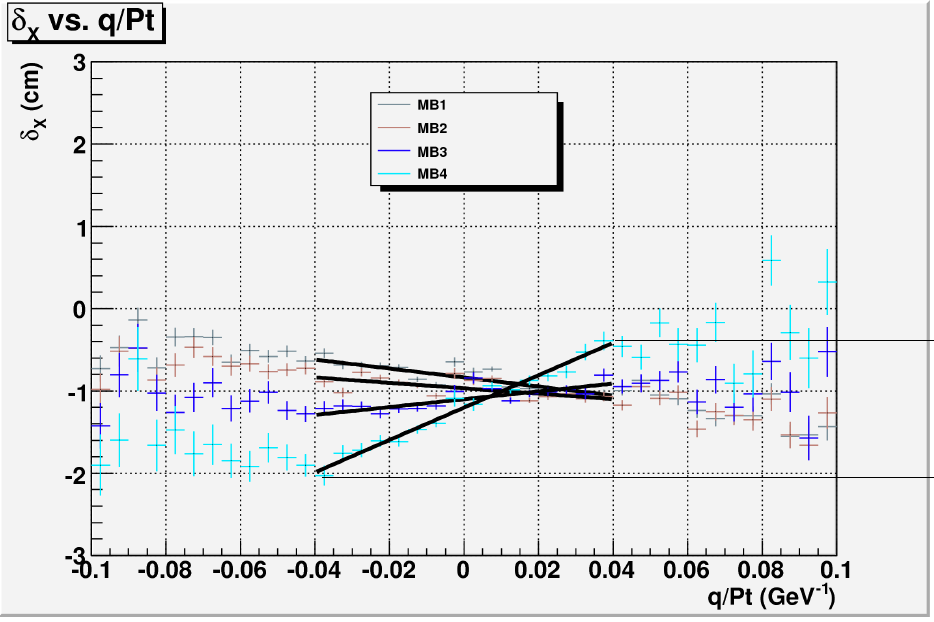
\includegraphics[width=\linewidth]{pmartinez.png}

\column{0.5\linewidth}

\vspace{-3.2 cm}
\begin{itemize}
\item $r\phi$ residual as a function of track curvature ($q/p_T$) is linear if $B_z$ is mismodelled
\item quadratic in extrapolation length ($\ell$)
\item charge confusion with charge ratio $\ne$ 1 distorts linear dependence at small $|q/p_T|$ if extrapolation length is large

\vspace{-0.2 cm}
\begin{itemize}
\item use residuals differences
\end{itemize}

\item scattering distorts linear dependence at \mbox{large $|q/p_T|$\hspace{-1 cm}}
\end{itemize}

\vspace{-1.5 cm}
\mbox{ }
\end{columns}
\end{frame}

\begin{frame}
\frametitle{Fit function for residuals}

\vspace{0.2 cm}
\begin{columns}
\column{0.65\linewidth}

\vspace{-0.35 cm}
\begin{itemize}
\item Scattering processes have power-law distributions, while experimental resolution is Gaussian

\item ``Peak'' of residuals distribution used in alignment comes from an unbinned fit to Lorentzian-Gaussian convolution

\vspace{-0.5 cm}
\begin{multline*}
f(x) = \int_{-\infty}^\infty \frac{1}{\pi}\frac{\Gamma/2}{(x - \xi)^2 + (\Gamma/2)^2} \times \\
\frac{1}{\sqrt{2\pi} \sigma} \exp\left(\frac{-\xi^2}{2 \sigma^2}\right) \, d\xi
\end{multline*}

\item Regular mean ($\sum x_i/N$) = center of an unbinned Gaussian fit; this just adds tails
\begin{itemize}
\item outliers matter less in peak-finding
\end{itemize}

\item For $B_z$ measurement, make peak a linear function of $q/p_T$ \mbox{(red is crest of 2-D fit)\hspace{-1 cm}}
\end{itemize}

\column{0.35\linewidth}

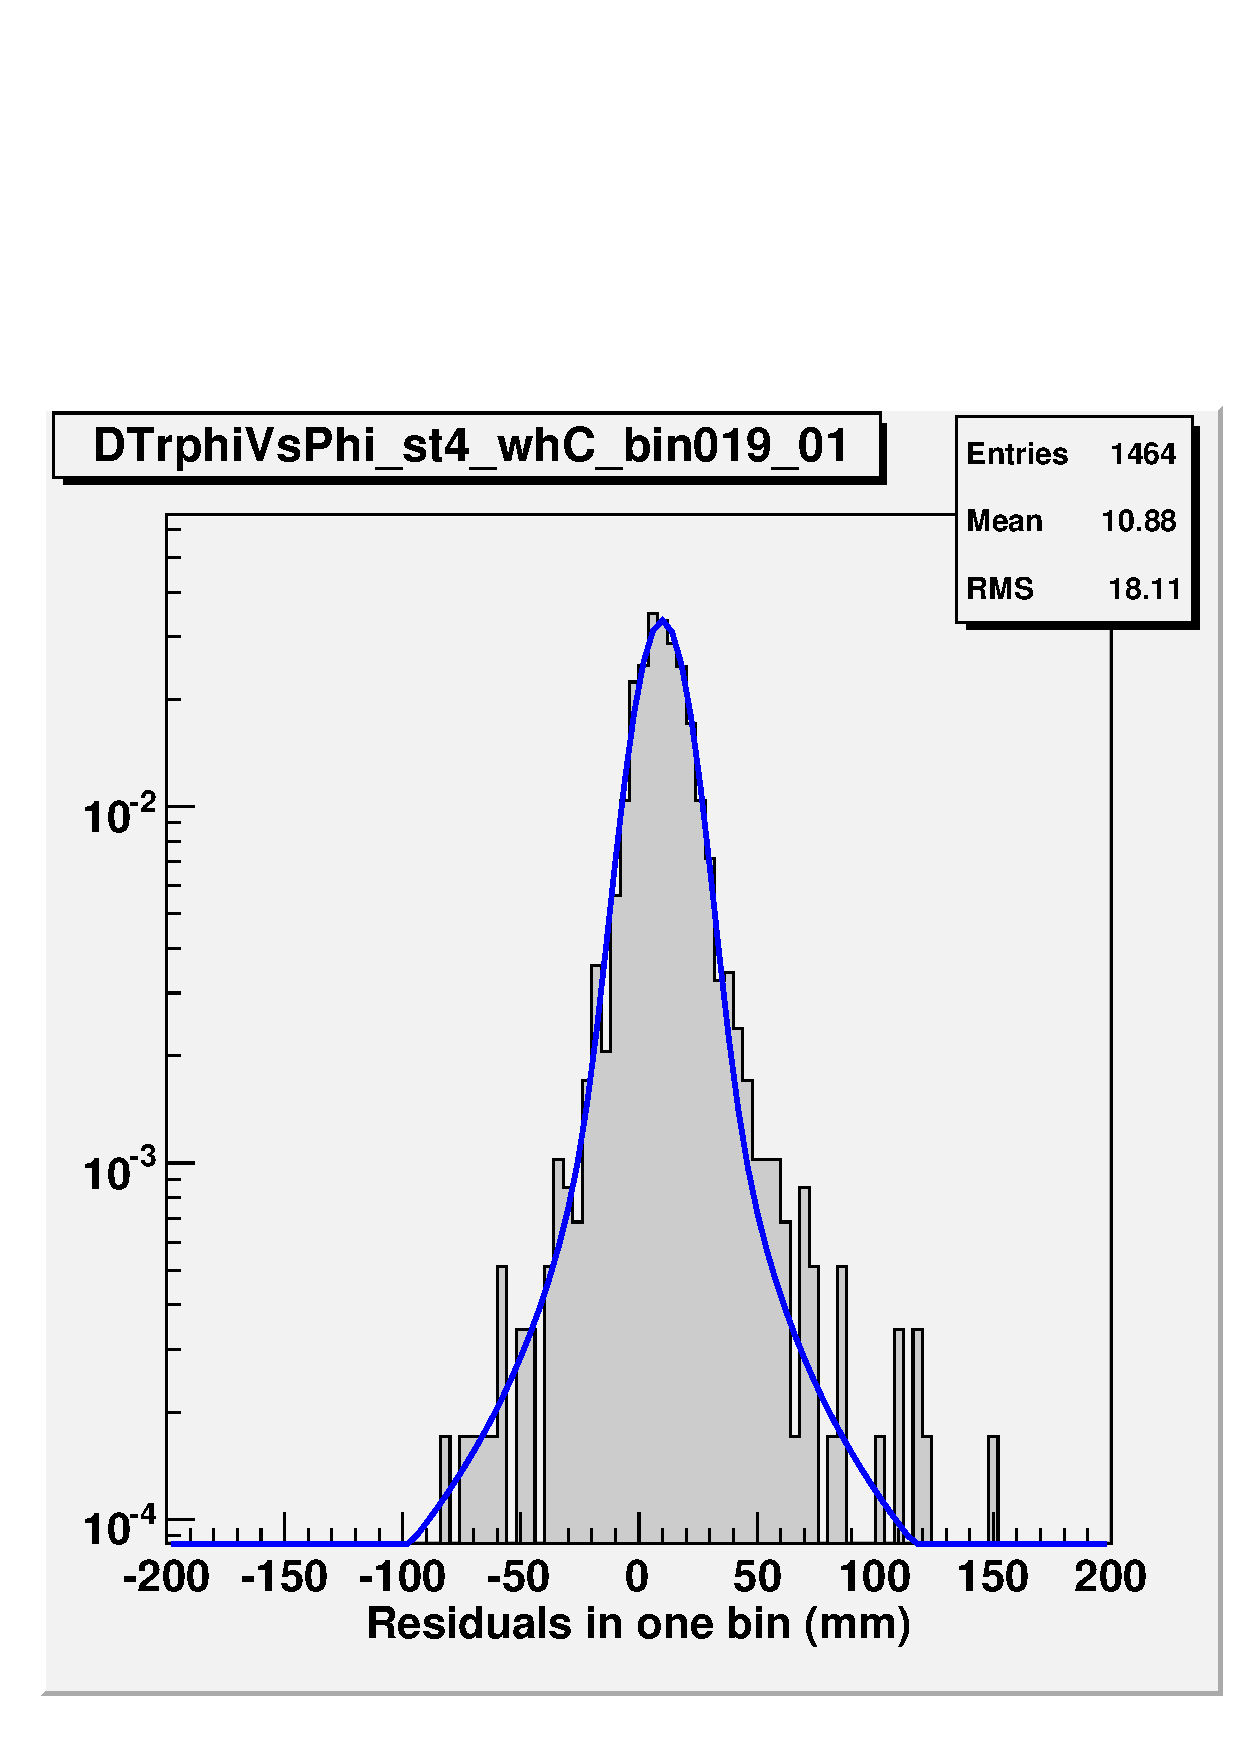
\includegraphics[width=\linewidth]{fitfunction.pdf}

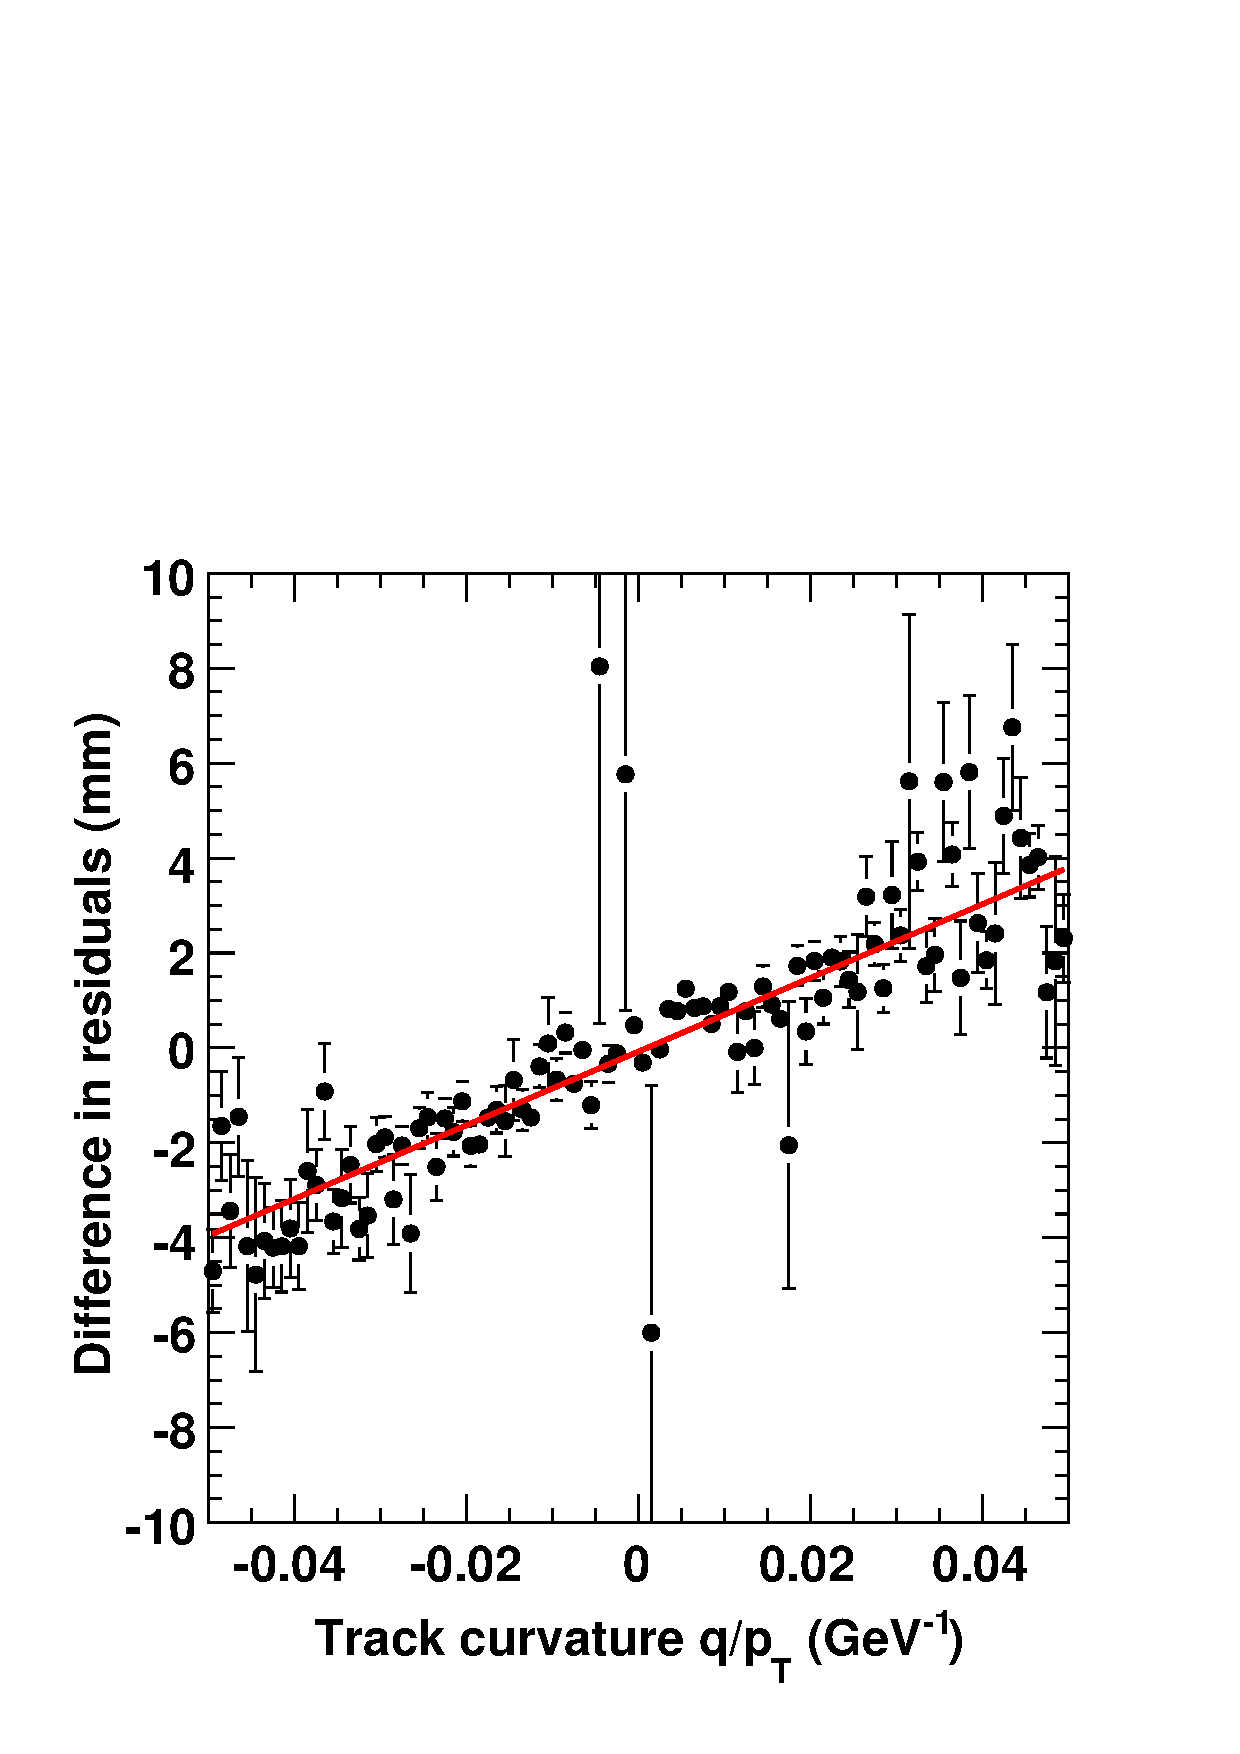
\includegraphics[width=\linewidth]{demo_qoverpt.pdf}
\end{columns}
\end{frame}

\begin{frame}
\frametitle{$B_z$ error between stations \only<1>{1\&2}\only<2>{2\&3}\only<3>{3\&4}}

\begin{itemize}
\item Points calculated from unbinned 2-D fits to $r\phi$ residuals and $q/pT$
\item Assumptions: $B_x = B_y = 0$, uniform $B_z$ between stations, \mbox{no $dE/dx$ error\hspace{-1 cm}}
\item Shown as a function of $\phi$, $z$ (same magnitude as combined fit)
\begin{itemize}
\item largest $B_z$ errors seem to be 8\% between stations 3\&4 \\ \mbox{\scriptsize (dataset is all 3.8~T: 66604-66904, 67126-67225, 67534-67647, 67680-68087)\hspace{-1 cm}}
\item slight wheel-by-wheel dependence?  or $dE/dx$ error?
\end{itemize}
\end{itemize}

\only<1>{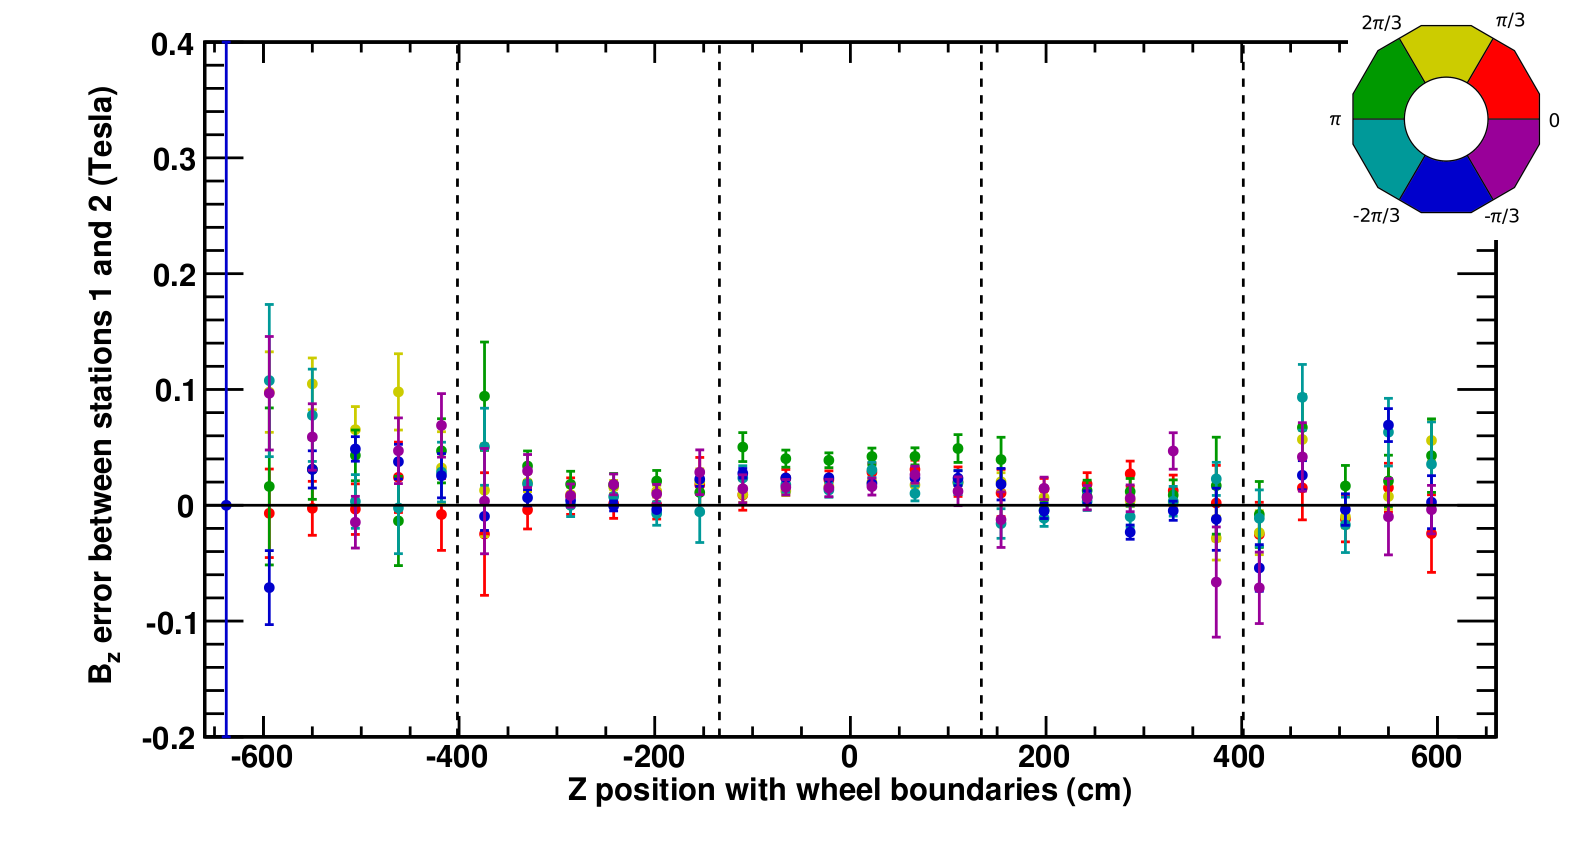
\includegraphics[width=0.95\linewidth]{berror12.png}}
\only<2>{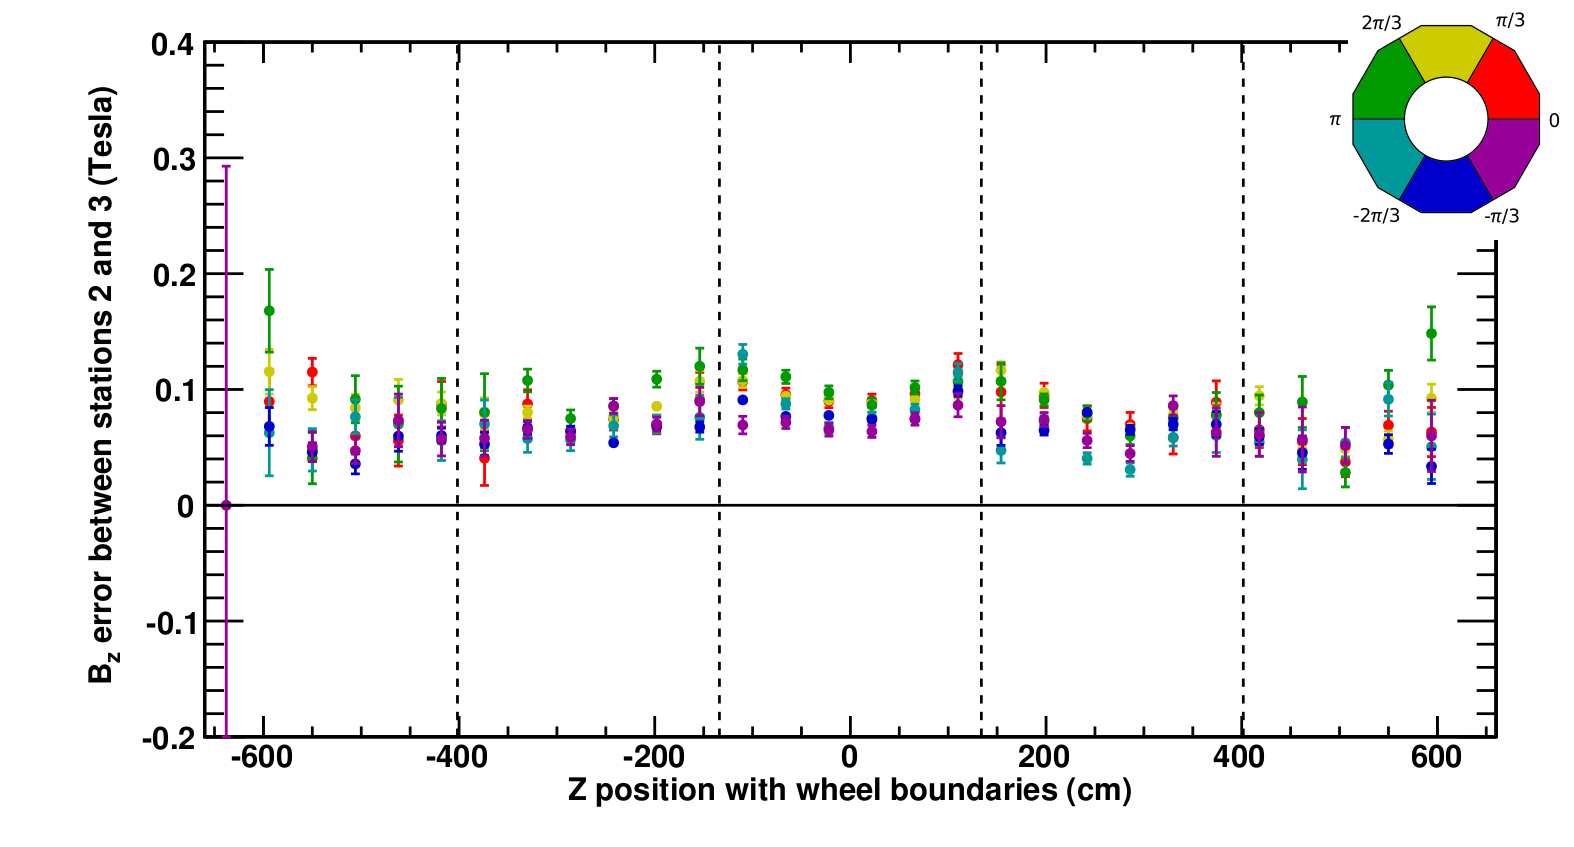
\includegraphics[width=0.95\linewidth]{berror23.png}}
\only<3>{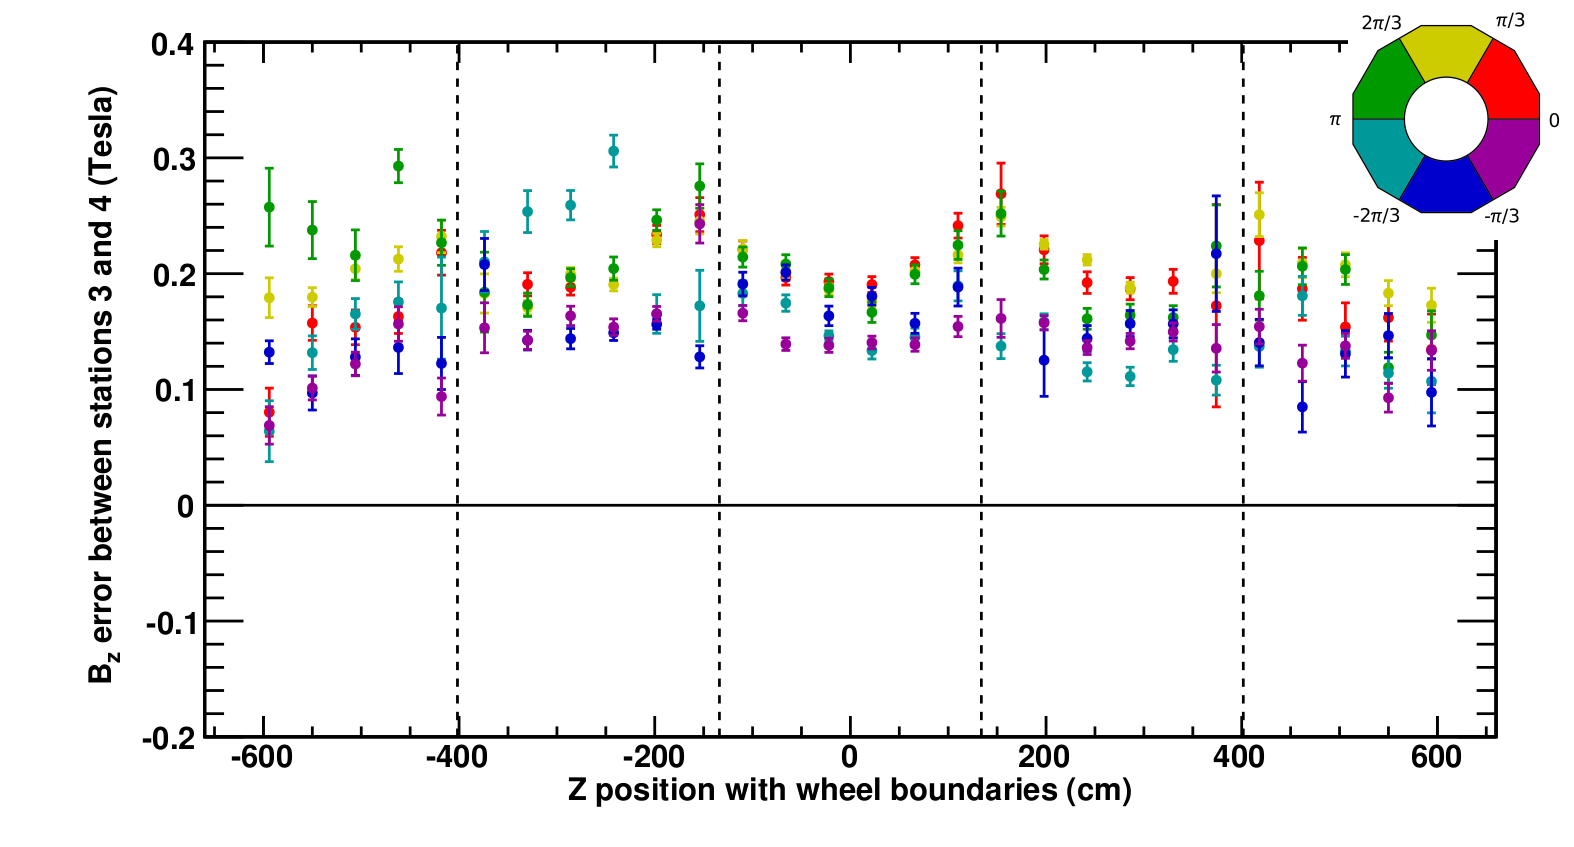
\includegraphics[width=0.95\linewidth]{berror34.png}}

\end{frame}

%% \section*{First section}
%% \begin{frame}
%% \begin{center}
%% \Huge \textcolor{blue}{First section}
%% \end{center}
%% \end{frame}

\begin{frame}
\frametitle{Conclusions}
\begin{itemize}\setlength{\itemsep}{0.5 cm}
\item Misalignments and $\vec{B}$-field errors can be disentangled
\item Alignment validation plots quantify systematic error from $\vec{B}$-field (times a large factor) in millimeters
\item Residuals differences localize $\vec{B}$ error between stations, rather than integrated along the whole track
\item $B_z$ error in Tesla can be calculated from linear dependence in $r\phi$ residuals vs.\ $q/p_T$
\item Largest $B_z$ errors seem to be only 8\% of 3.8~T
\end{itemize}
\label{numpages}
\end{frame}

\end{document}
